\chapter{Implementazione e Risultati}
Andremo ora a soffermarci sull'esperienza diretta avuta sull'approccio alle tecnologie descritte precedentemente nel capitolo due, andando a definire delle implementazioni concrete su casi d'uso descritti nel capitolo quattro. Ci soffermeremo solamente su come le varie componenti comunichino tra di loro con la blockchain alla base dell'architettura. Descriveremo l'implementazione dei vari strati andando a specificare le scelte implementative effettuate nei due casi d'uso concretizzati in fase di progettazione. Concluderemo con la fase di raffinamento dei prototipi in modo da poter rispettare i criteri prefissati in fase progettuale andando a documentare passo dopo passo attraverso i principali snippet di codice che sono alle fondamenta di alcuni concetti funzionali del progetto. Il contesto su cui si concentra questo capitolo è basato solamente sull'implementazione delle componenti sviluppate singolarmente specificate nei contributi individuali all'interno del capitolo quattro.
\section{Client}
Sotto un punto di vista delle applicazioni rappresentanti data consumer o service provider, ci siamo concentrati sull'implementazione dei vari client legati ad alcuni attori andando a concentrarci sulla formattazione dei dati secondo la visione proposta dai server REST definita in back-end. Inoltre, si è aggiunto un ulteriore livello di protezione andando a controllare la formattazione e la correttezza dell'input in modo da evitare di generare delle request non valide, questo approccio di controllo ha lo scopo di allegerire il carico di lavoro del thread in event loop sul server REST.
\subsection{Front-End implementato nel contesto Healthcare}
Nel contesto sanitario, l'implementazione front-end si è concentrato sullo sviluppo dell'interfaccia grafica e sulla rappresentazione dei servizi offerte all'interno delle applicazioni in possesso degli attori principali del prototipo (Paziente, Centro Medico e Ospedale). Si sono sviluppate due applicazioni di tipo mobile, una per il paziente e una per l'ospedale, in cui poter eseguire tutte le funzionalità descritte in fase di progettazione. I miei contributi in questo strato di progettazione si sono concentrati sul centro medico che, invece, dispone di un'implementazione più semplice, basata su un'applicazione web che visualizzava un insieme di dati estrapolati dallo stato globale del ledger. Tali dati sono resi visibili al centro medico mediante i permessi di accesso propri della seconda organizzazione della blockchain. La struttura dell'applicazione front-end ricopre un'interfacciamento verso il server REST attraverso l'utilizzo di Servlet. Le Servlet non fanno altro che stabilire un canale con il server REST, inviare le richieste formattate in JSON e inoltrare le risposte all'interno della sessione dell'applicazione, di seguito riportiamo uno snippet di codice in Java inerente alla creazione della connessione per l'invocazione di un servizio di aggiornamento delle terapie della collezione riferita ai dati sensibili di un paziente sul server REST dedicato alla seconda organizzazione della blockchain:
\begin{figure}[h]
    \centering
    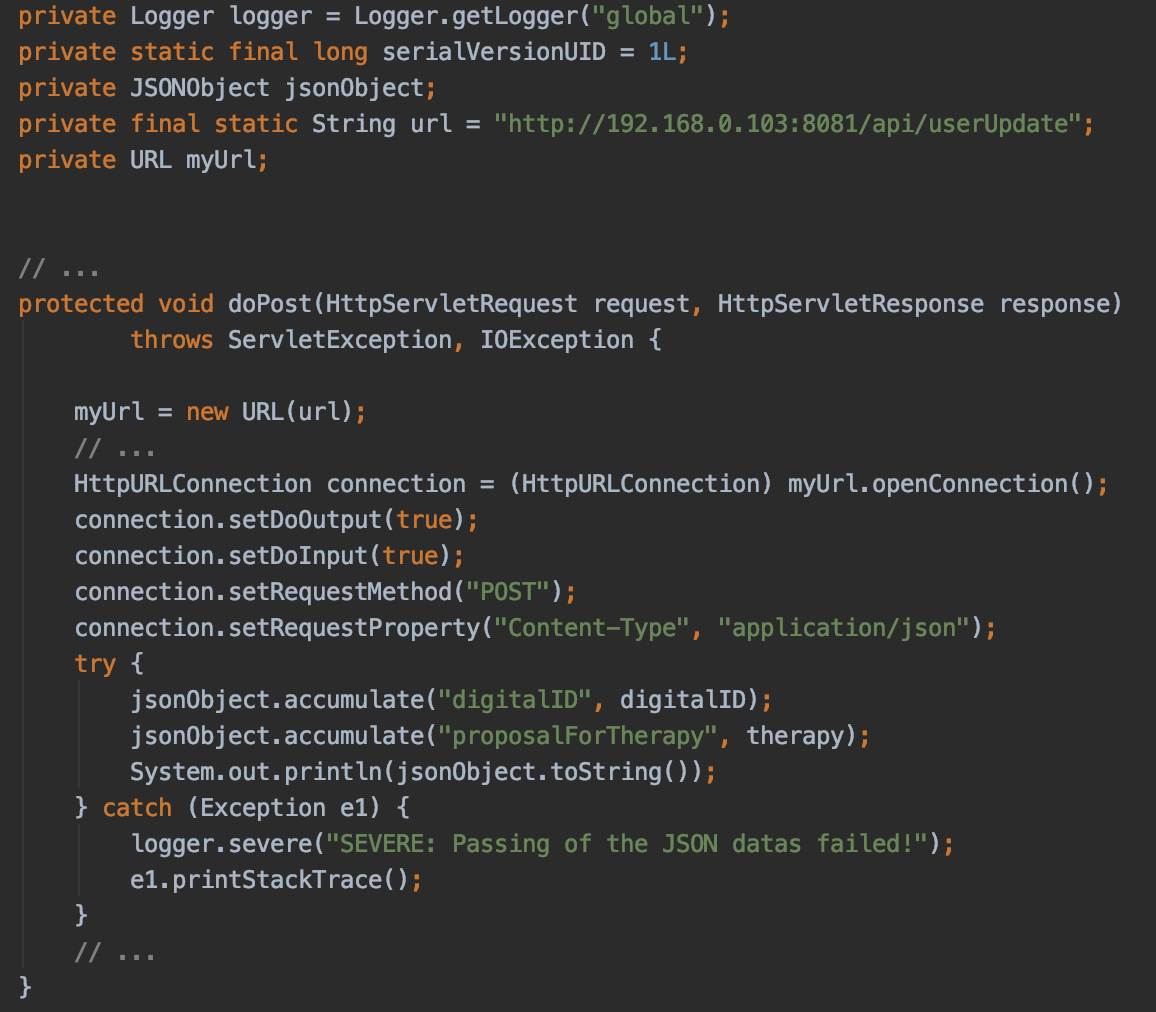
\includegraphics[width=0.6\textwidth]{img/connection_healthcare.png}
    \caption{Approssimazione dell'apertura di una connessione con il server REST all'indirizzo}
    \label{fig:connection_healthcare}
\end{figure}
\newpage
In seguito alla creazione di una connessione, si definisce un oggetto JSON da inviare, nel caso dell'esempio si invia una stringa rappresentante una proposta di terapia per un particolare paziente identificato da un UUID:
\begin{figure}[h]
    \centering
    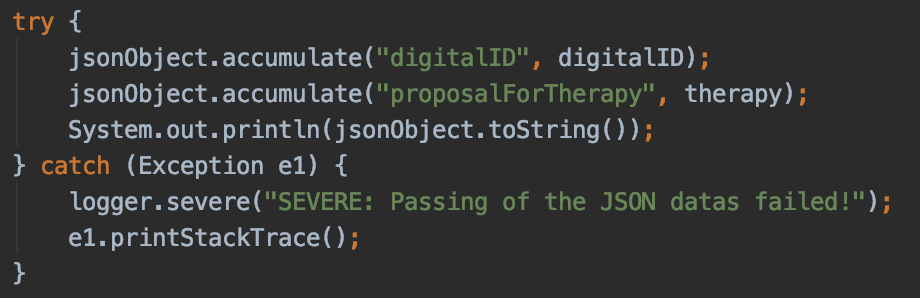
\includegraphics[width=1\textwidth]{img/json_object.png}
    \caption{Costruzione dell'oggetto JSON da inviare ad una request verso un server REST}
    \label{fig:json_request}
\end{figure}
In seguito dell'inoltro della request formattata in JSON, la Servlet attende una risposta dal flusso di input della connessione. Nel caso in esempio, si ha una stringa che rappresenta un array di JSON corrispondente a una serie di entità di una collezione mantenuta all'interno dello stato globale del ledger. La gestione della risposta è simile a come segue:
\begin{figure}[h]
    \centering
    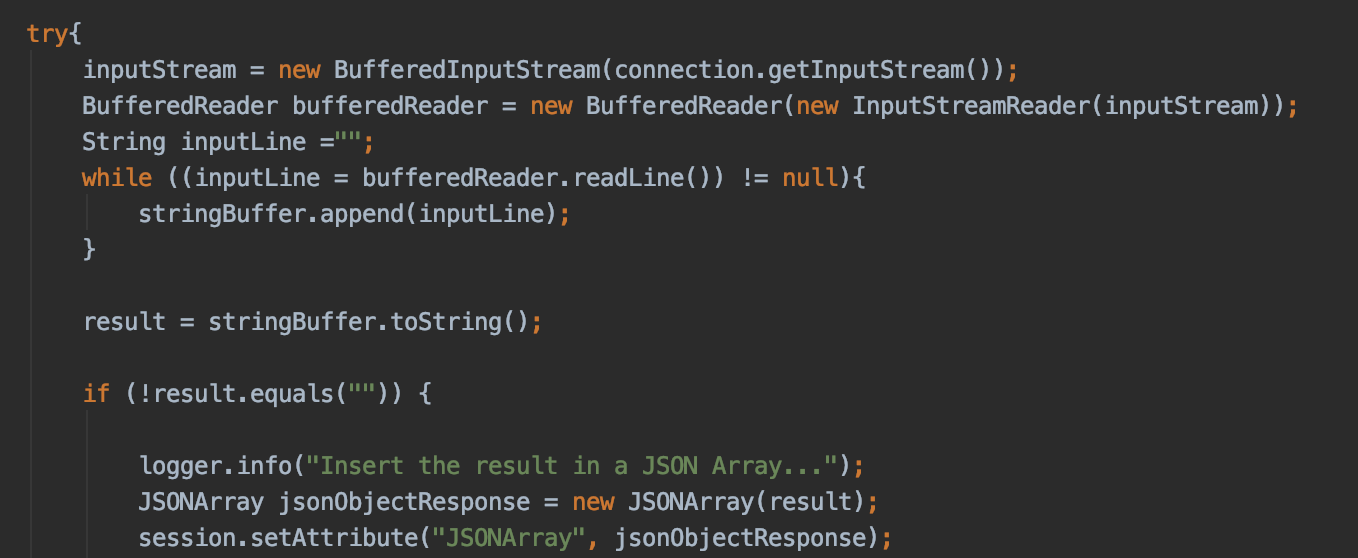
\includegraphics[width=1\textwidth]{img/response_string.png}
    \caption{Formattazione ed inserimento della response della REST API all'interno della sessione del client}
    \label{fig:json_response}
\end{figure}
Nei snippet di codice sopra riportati si può vedere come l'utilità della servlet sia principalmente quella di stabilire un canale di comunicazione con il server andando a formattare in JSON i dati di input e inserire in sessione i dati di output in modo da poter essere visibili e utilizzabili all'interno delle pagine web visualizzate. Per tutte le altre operazioni inerenti alle applicazioni in front-end si ha, come base, quella dell'esempio di modifica riportato in precedenza. 
\subsection{Front-End implementato nel contesto Automotive}
Nel contesto Automotive, il lato front-end comprende un insieme di dashboard e un simulatore di aggiornamento dei dati parametrici sulle collezioni rappresentanti le componenti dell'auto sotto monitoraggio. L'aggiornamento simulato prevede l'inserimento di una serie di valori che andranno ad aggiornare un'entità dello stato globale del ledger creando, a una determinata frequenza, delle transazioni che vengono inserite all'interno di nuovi blocchi collegati alla blockchain. Le dashboard leggono, contemporaneamente, i dati su una singola componente o di tutte le componenti di un'auto a una determinata frequenza. Dentro questo paragrafo andremo ad analizzare solamente un esempio d'implementazione relative alle funzionalità delle dashboard. Ogni dashboard ha una struttura simile, le funzionalità si distinguono principalmente per i tipi di dati che richiedono andando a mantenere una medesima logica funzionale. Possiamo ora analizzare un esempio d'implementazione per la richiesta e il prelievo dei dati andandone a considerare la loro lettura inerenti alle informazioni legate al motore di un'auto identificata tramite un UUID.
\begin{figure}[h]
    \centering
    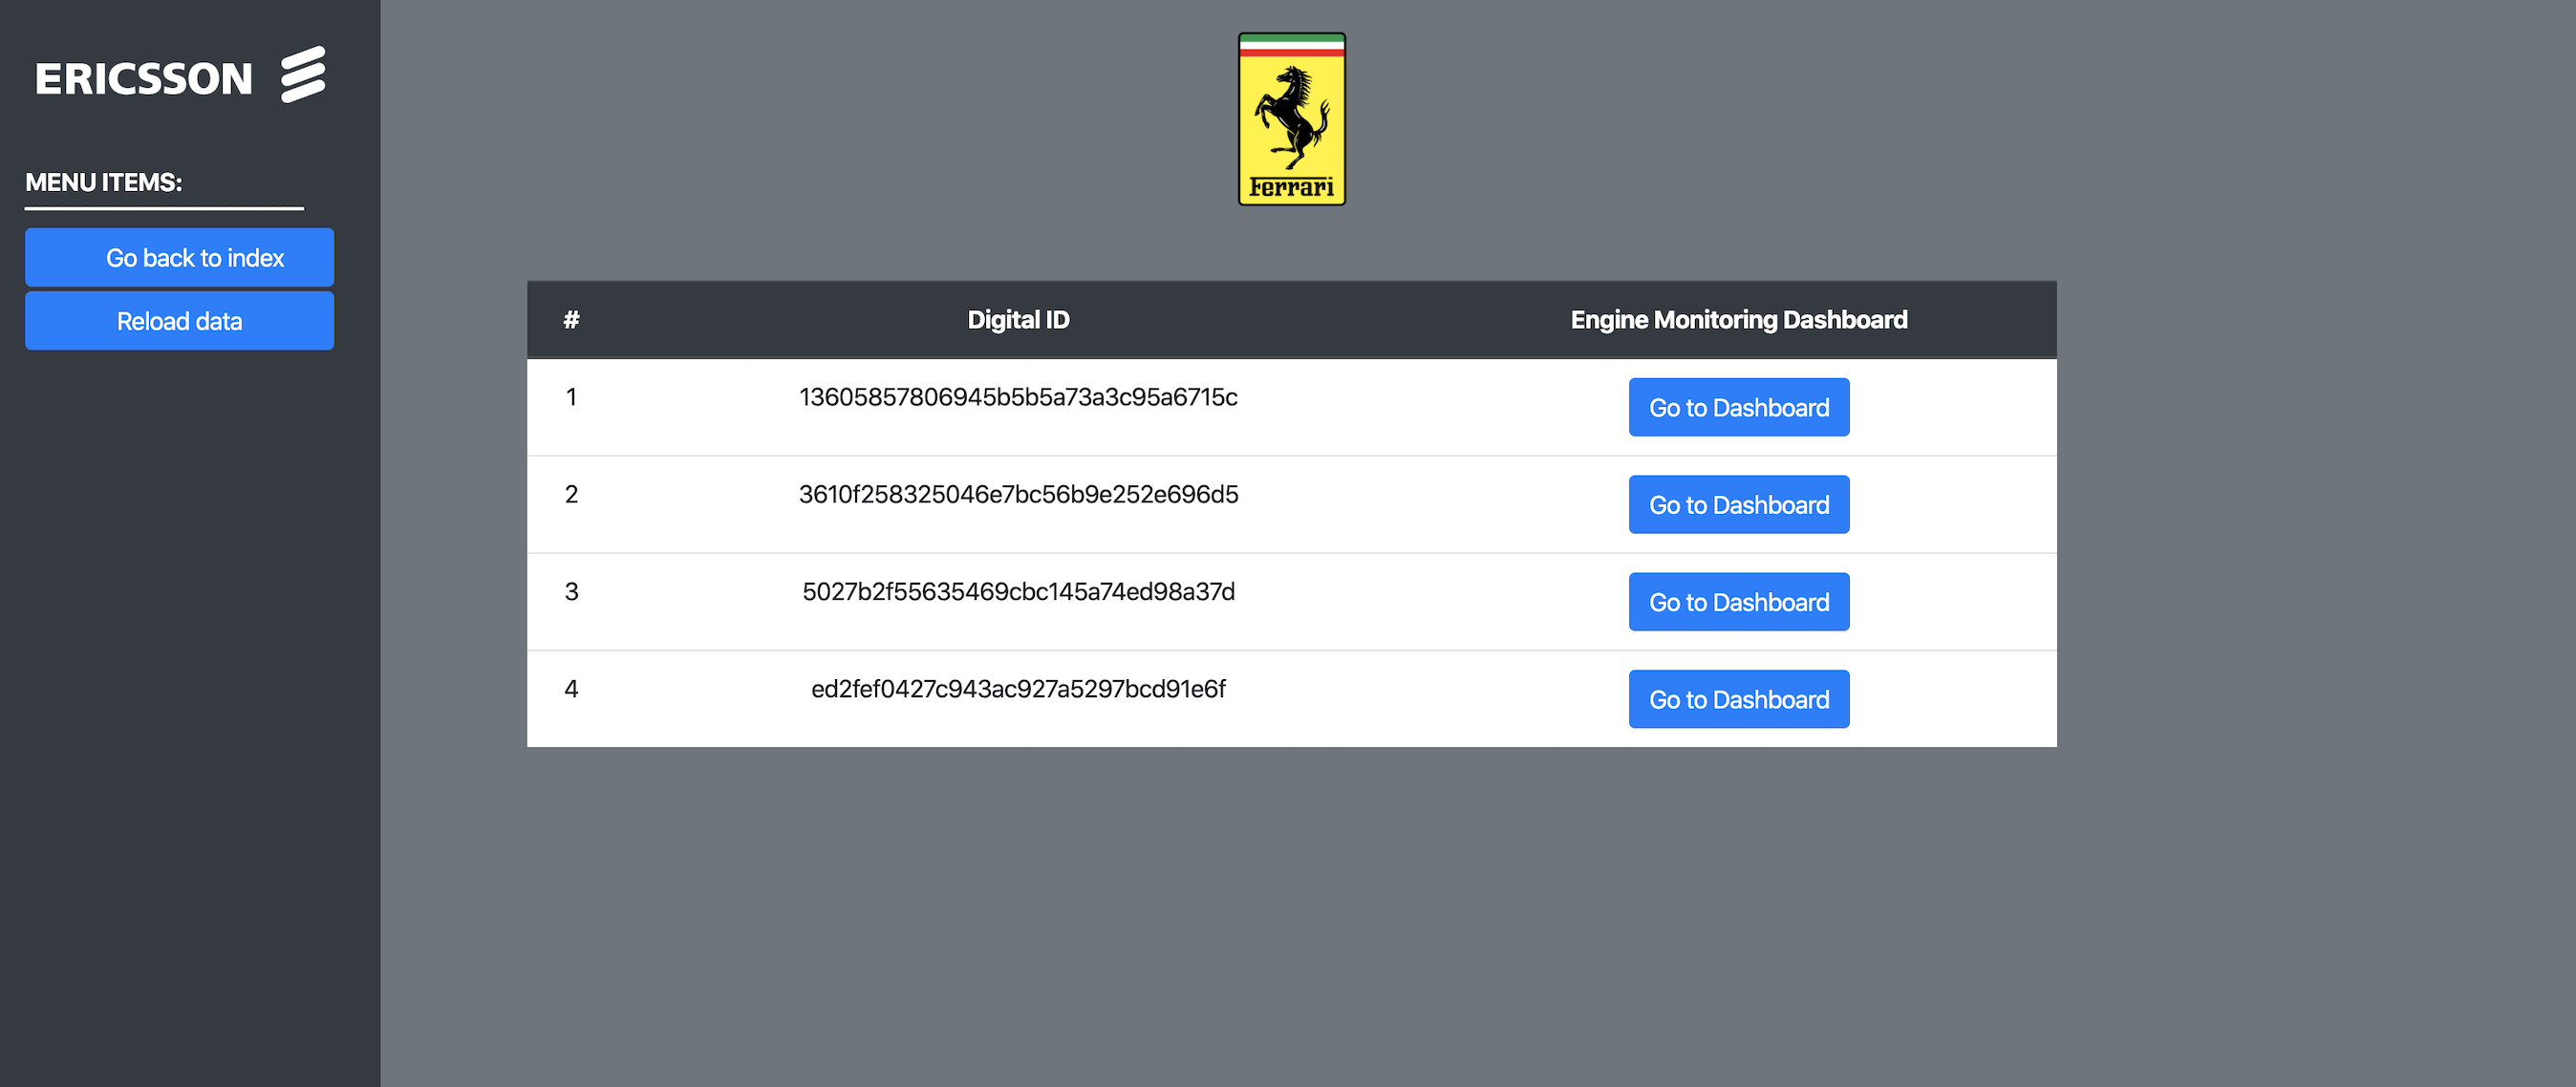
\includegraphics[width=1\textwidth]{img/table_engine_dash.png}
    \caption{Tabelle delle varie entità registrate all'interno dello stato globale della blockchain}
    \label{fig:table_dash}
\end{figure}
La comunicazione con il server REST è assegnata a una Servlet d'interfacciamento che si occupa di gestire i dati di sessione, creare una connessione e formattare le informazioni di input e di output. La logica di business propria della Servlet è simile al caso d'uso sanitario. L'unica differenza si ha per la gestione della sessione che non prevedono l'inserimento di una lista di dati letti dallo stato globale del ledger della blockchain, ma gli stati delle informazioni "storiche" mantenute negli ultimi cinque blocchi della catena, poiché bisogna ottenere una visione di confronto tra le ultime cinque letture. Tutti i dati monitorati vengono salvati all'interno di una storia delle informazioni provvisorie e proprie della sessione di un client:
\begin{figure}[h]
    \centering
    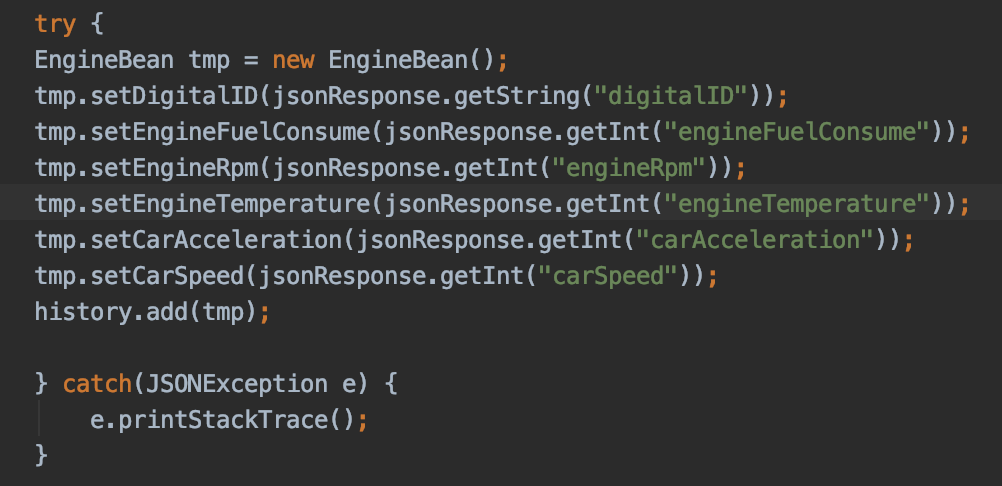
\includegraphics[width=1\textwidth]{img/history_screen.png}
    \caption{Salvataggio in sessione dei valori JSON di ritorno dal server REST}
    \label{fig:session_history}
\end{figure}
Si è scelto in fase implementativa di non disporre di meccanismi interni al chaincode per estrapolare i dati volta per volta dagli ultimi cinque blocchi della catena per l'assenza di una chiamata a sistema relativa al prelievo degli stati mantenuti nella storia del ledger. Gli ultimi aggiornamenti della libreria shim dispongono, nelle proprie API, una funzione denominata "getHistoryByKey" in cui preleva un insieme di coppie di valori relative ai dati della storia trasferita insieme ai timestamp del blocco di appartenza relativi a un entità definita dal valore della chiave passata in input. Di seguito mostriamo la dashboard finale corrispondente al monitoraggio della temperatura, del consumo di carburante di un motore e gli RPM dell'auto sotto analisi:
\newpage
\begin{figure}[h]
    \centering
    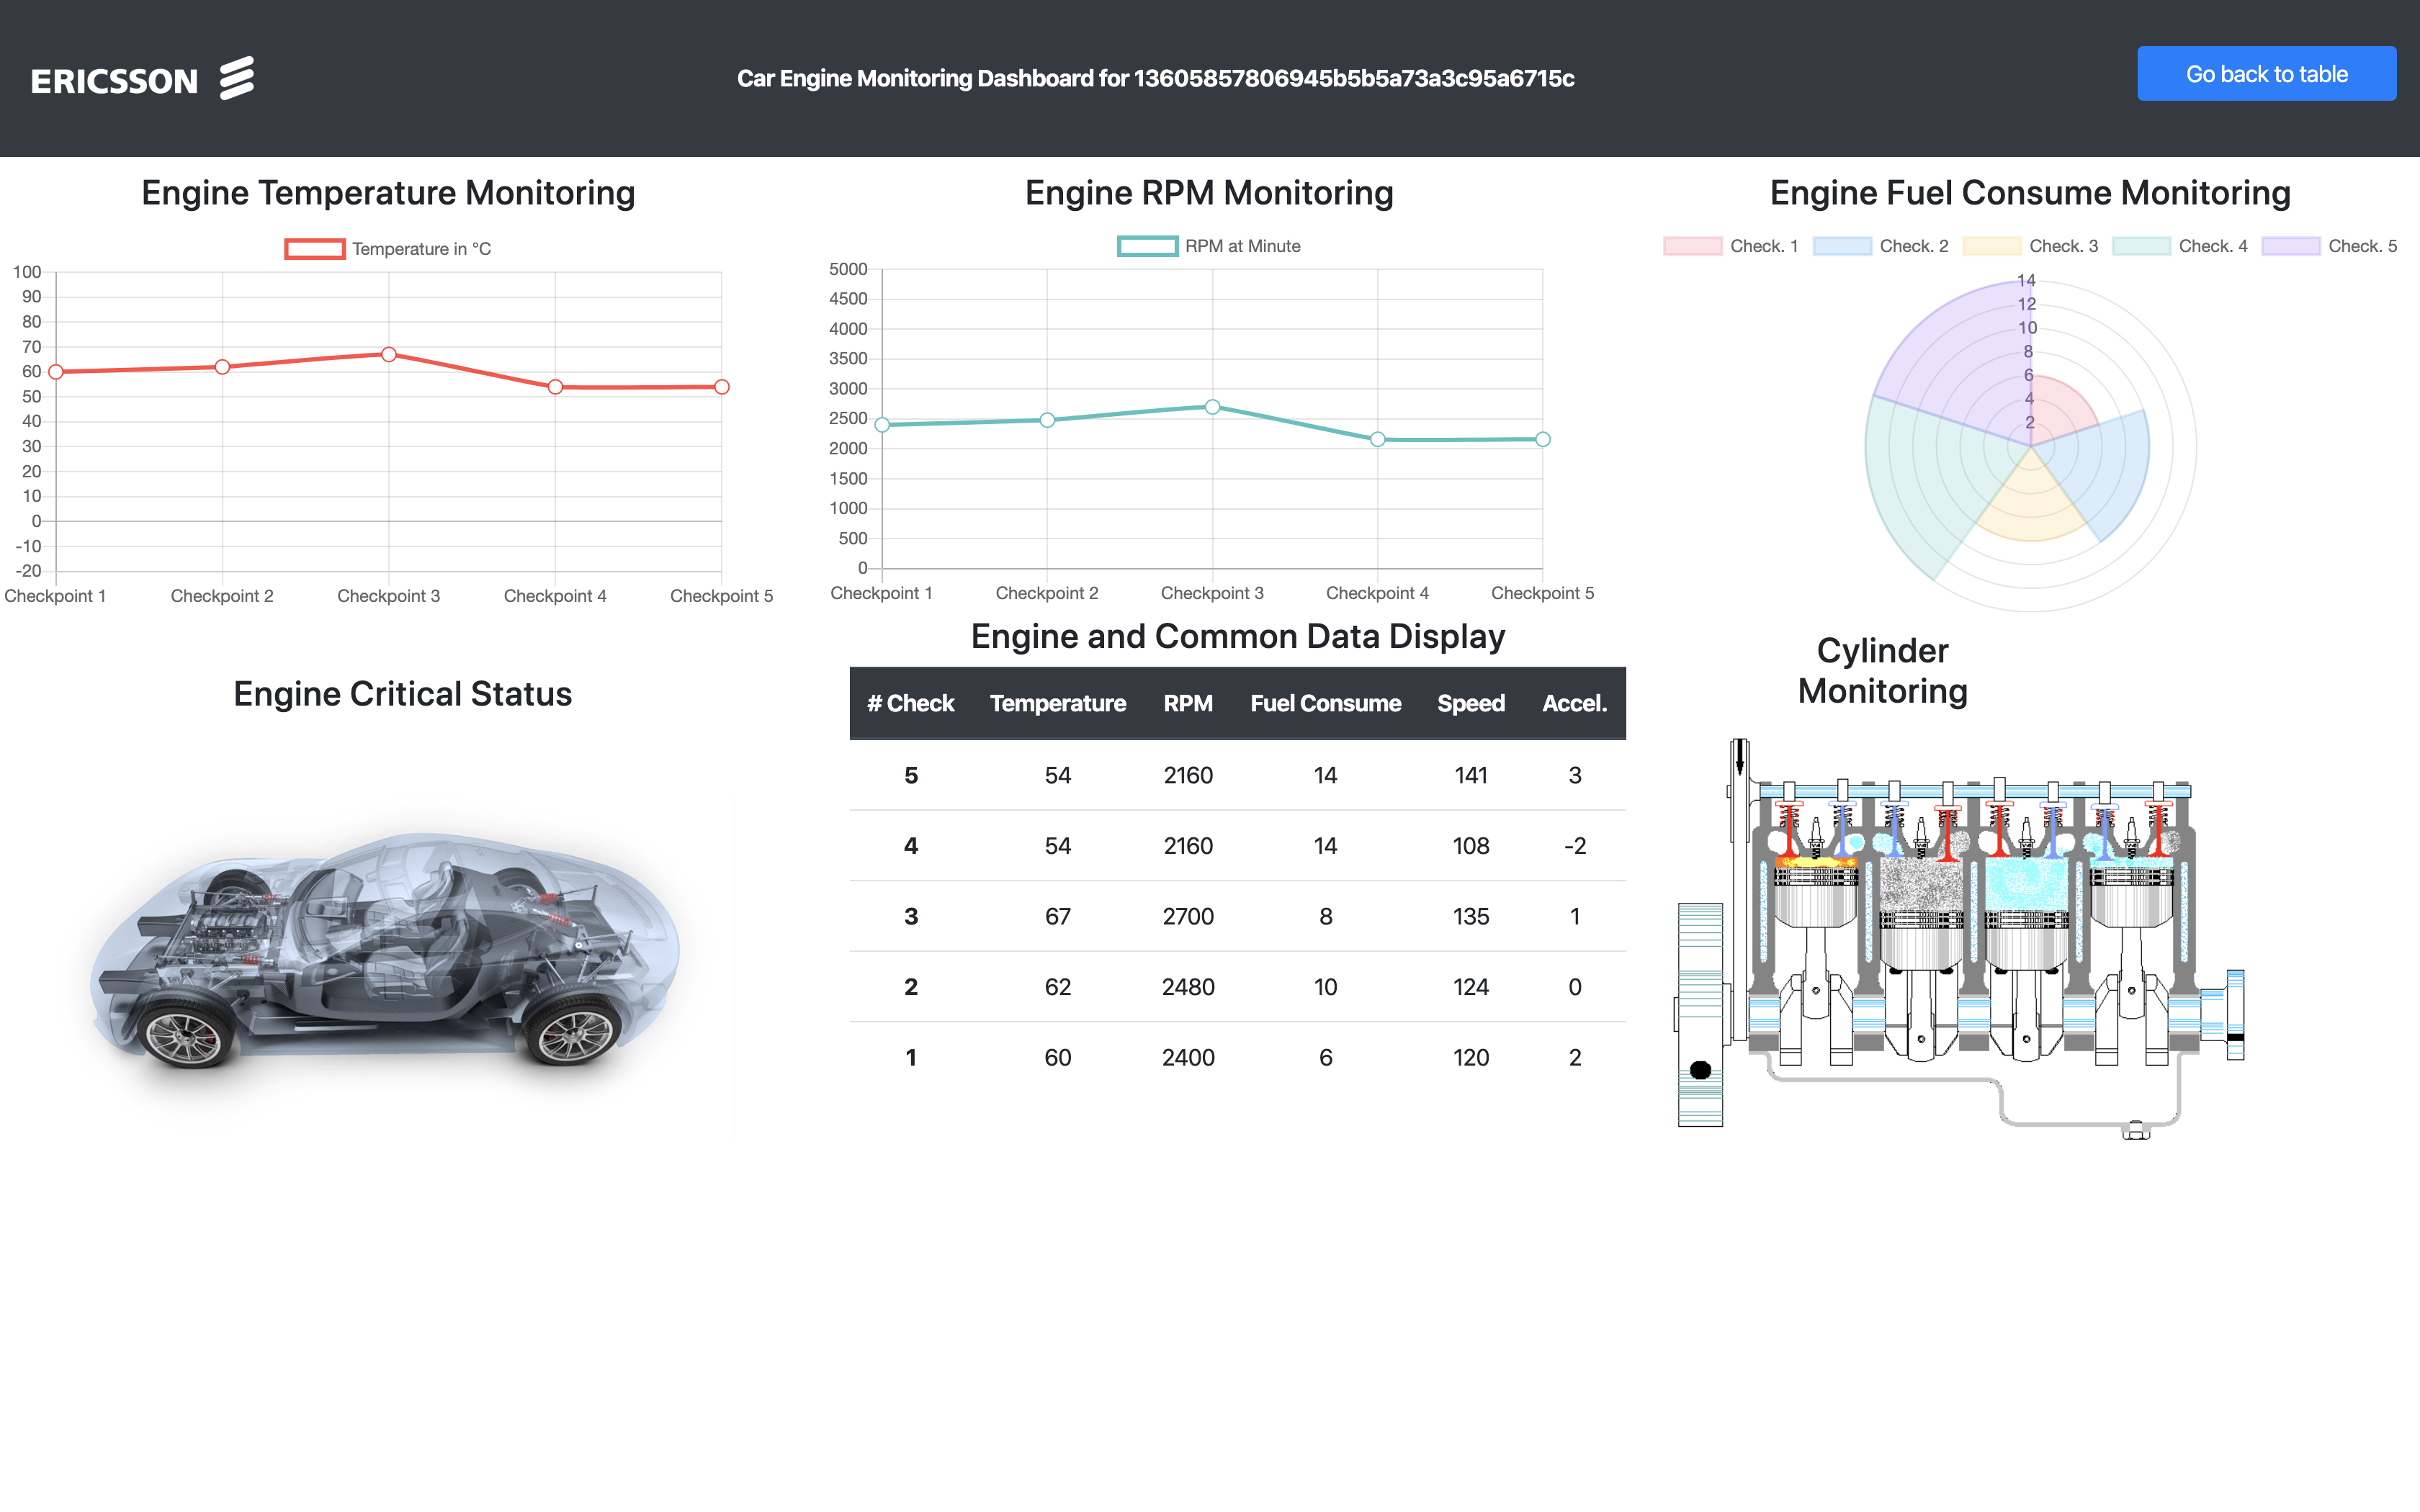
\includegraphics[width=1\textwidth]{img/engine_monitoring.png}
    \caption{Dashboard di monitoraggio per il motore di un'auto}
    \label{fig:dashboard_automotive}
\end{figure}
Le difficoltà maggiori che si sono riscontrate si basano sul dover adattare la frequenza di monitoraggio con la latenza dell'architettura poichè, per mantenere affidabilità, la blockchain ha bisogno di validare ogni blocco aggiunto dal simulatore. Tale meccanismo, anche se ad alte prestazioni, crea latenza all'interno della rete e, in fase di lettura, bisogna diminuire la frequenza per poter leggere i dati aggiornati in maniera corretta. 
\newpage
\section{Back-End}
L'implementazione delle componenti back-end si è concentrata sulla creazione di server REST che forniscono un'interfaccia pubblica di gestione per le varie funzioni invocabili di un chaincode installato sul canale della blockchain sottostante. Questa caratteristica è comune a entrambi i prototipi sviluppati che variano la propria interfaccia pubblica per: 
\begin{itemize}
    \item Funzione da invocare all'interno del chaincode
    \item Input da passare all'invocazione della funzione
    \item Output restituito
\end{itemize}
Le varie REST API che compongono il server definiscono tutte le operazioni che bisogna effettuare all'interno delle collezioni dello stato globale del ledger della blockchain offrendo un livello logico direttamente utilizzabile ai client. Se, però, i client non sono autorizzati a effettuare particolari funzioni del chaincode dello strato sottostante, la chiamata restituirà un errore di autorizzazione. Definiamo ora la struttura interna dell'implementazione di uno dei server REST implementati soffermandoci sulle operazioni d'interazione con la blockchain sottostante. 
I server REST sono basati sul framework Express.js per le operazioni di connessione asincrona sulle chiamate alle API offerte dal REST web service che si vuole creare. Utilizzeremo anche alcuni SDK (Software Developer Kit) tra cui "fabric-client" per definire le interazioni tra il server e le componenti della blockchain Fabric e "body-parser" per la gestione della formattazione del corpo della request all'interno di un middleware. Tramite SDK specifici, possiamo manipolare entità e proprietà proprie della blockchain Fabric, all'interno dell'implementazione si è stabilito, per ogni server, un peer di riferimento tra quelli dell'organizzazione su cui si interfaccia, l'orderer e il canale dell'architettura per la validazione e la sottomissione delle varie transazioni che si andranno a creare. 
Di seguito riportiamo il codice per l'instanziazione delle componenti logiche d'interazione con Fabric
\begin{figure}[h]
    \centering
    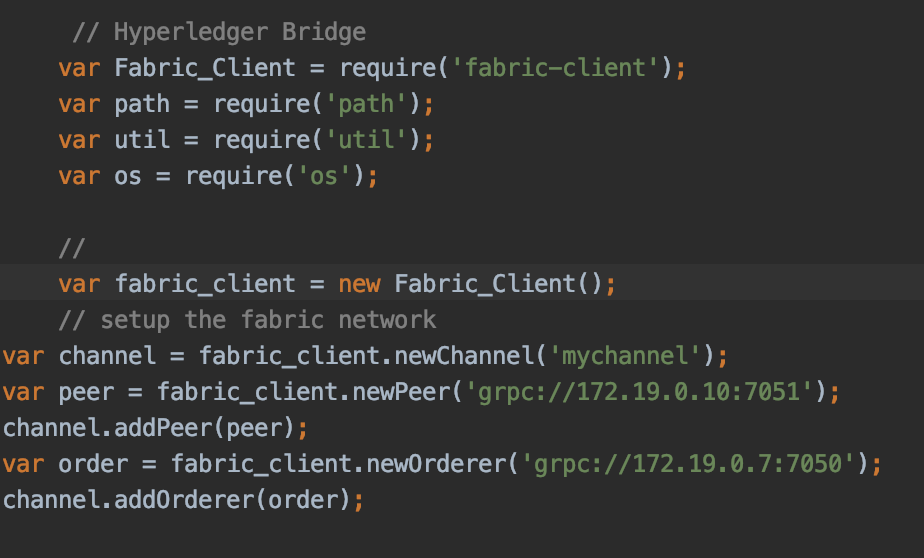
\includegraphics[width=1\textwidth]{img/express-comp-fabric.png}
    \caption{Snippet di codice per l'instanziazione delle componenti logiche di Fabric interessate nella comunicazione con il server REST}
    \label{snippet-comp-fabric}
\end{figure}
\newpage
Per mantenere la logica architetturale propria di Fabric, ogni REST API  deve poter rispettare le seguenti proprietà: 
\begin{enumerate}
    \item Bisogna adottare un meccanismo che richiami le CA di Fabric per mantenere i criteri di autenticazione e di autorizzazione.
    \item Prima di inviare una transazione che aggiorna lo stato globale del ledger della blockchain, bisogna inviare una proposta di transazione e gestire i possibili risultati del consenso. 
    \item Creare e gestire la transazione andando ad invocare una funzione del chaincode e propagare il risultato al client all'interno della response della REST API. 
\end{enumerate}
All'interno del prototipo, la logica di autenticazione prevede l'estrapolazione della chiavi di autenticazione all'interno di un wallet locale andando a richiamare un contesto legato ad un singolo utente, ciò sta a significare che ogni richiesta di transazione proveniente dal server REST e mantenuta all'interno del ledger di Fabric verrà segnata con la firma dell'utente del prototipo. 
\begin{figure}[h]
    \centering
    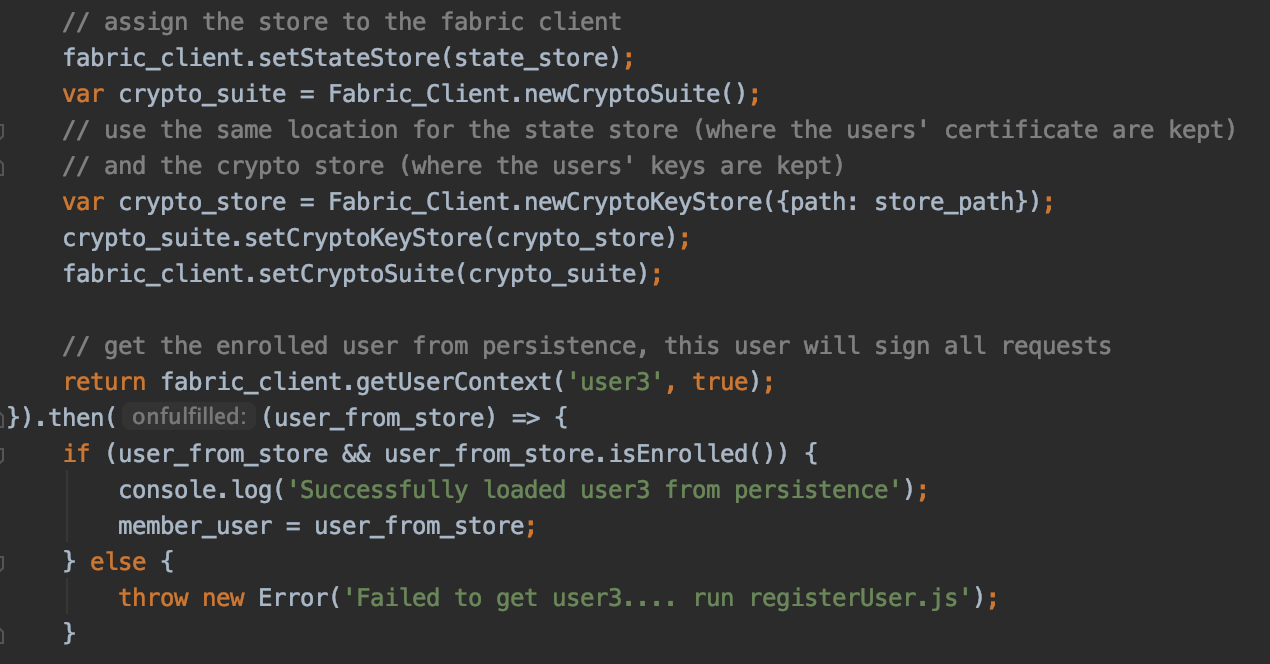
\includegraphics[width=1\textwidth]{img/aut-server.png}
    \caption{Snippet di codice l'autenticazione per la gestione delle signature di un'utente di esempio mantenuto in un wallet del prototipo}
    \label{autent-express-server}
\end{figure}
In seguito all'impostazione per rispettare il criterio di autenticazione, i server REST formattano la richiesta che andrà in input al chaincode in modo da poter invocare una specifica funzione andando a passare i parametri di input richiesti. Tale richiesta andrà ad essere inviata nella proposta di transazione e verificata nel seguente modo:

\begin{figure}[h]
    \centering
    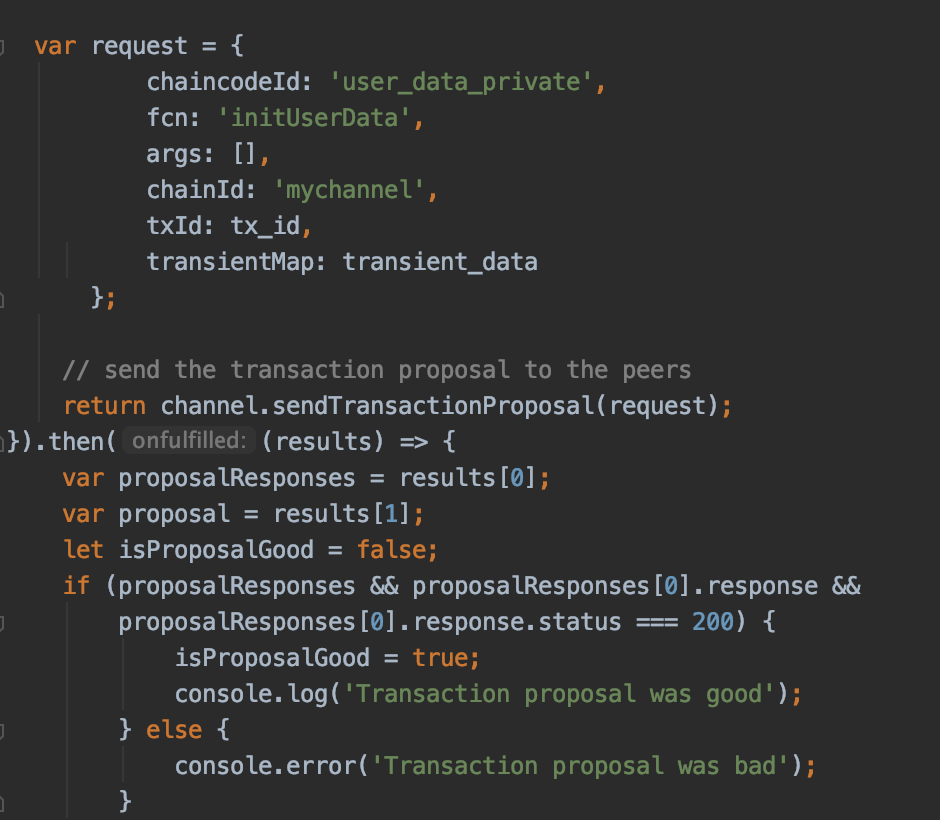
\includegraphics[width=0.5\textwidth]{img/proposal-request.png}
    \caption{Snippet di codice di gestione della proposta di transazione}
    \label{proposal-script}
\end{figure}
Se la proposta è andata a buon fine, viene definita una richiesta di transazione contente la risposta della proposta di transazione insieme ai dati di input e alle informazioni di invocazione. La richiesta di transazione viene inviata all'orderer per il commit della transazione in modo da effettuare l'aggiunta di un blocco di transazione che andrà ad aggiornare le istanze del ledger di ogni peer della blockchain. La transazione andrà a modificare lo stato globale delle istanze dei ledger dei peer della rete solamente se l'operazione è di scrittura. La REST API riceverà in risposta l'output della transazione e, a secondo se sia considerata valida o meno, verrà inoltrato una specifica risposta al client: 
\begin{figure}[h]
    \centering
    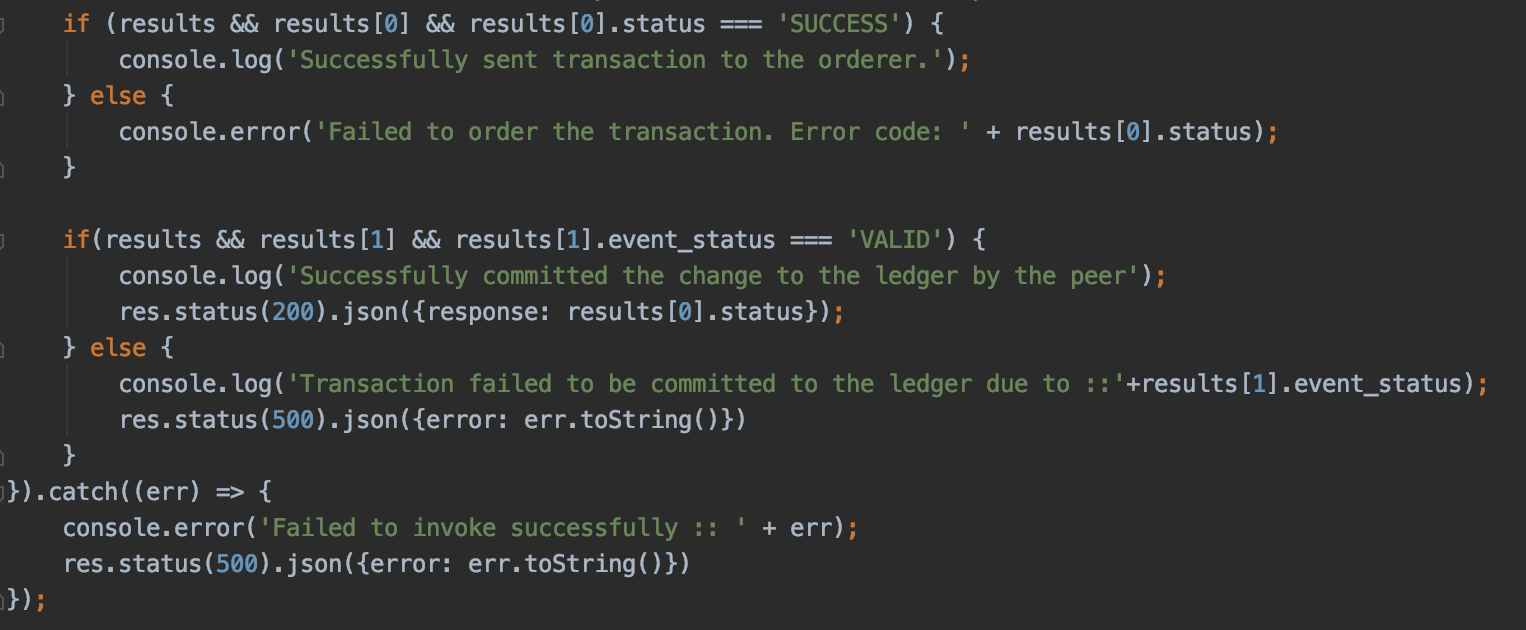
\includegraphics[width=1\textwidth]{img/response-result.png}
    \caption{Gestione della risposta ad una REST API}
    \label{result-script}
\end{figure}
\newpage
\section{Rete basata su Hyperledger Fabric}
All'interno di questo paragrafo andiamo a definire tutta la configurazione dell'architettura Fabric implementata all'interno dei prototipi. Poichè non vi è distinzione all'interno della struttura della blockchain tra i due prototipi implementati, non si avranno distinzione tra i due casi d'uso.
\subsection{Script di inizializzazione}
La rete su cui è basata la blockchain è formata da due organizzazioni, un canale, un orderer, quattro peer (due per ogni organizzazione), un interfaccia a riga di comando, un'istanza di un database di stato del leger basato su couchdb e due istanze dei chaincode montate su ogni organizzazione. La composizione dei container si basa sulla struttura del progetto "first-network" disponibile in open-source. 
\begin{figure}[h]
    \centering
    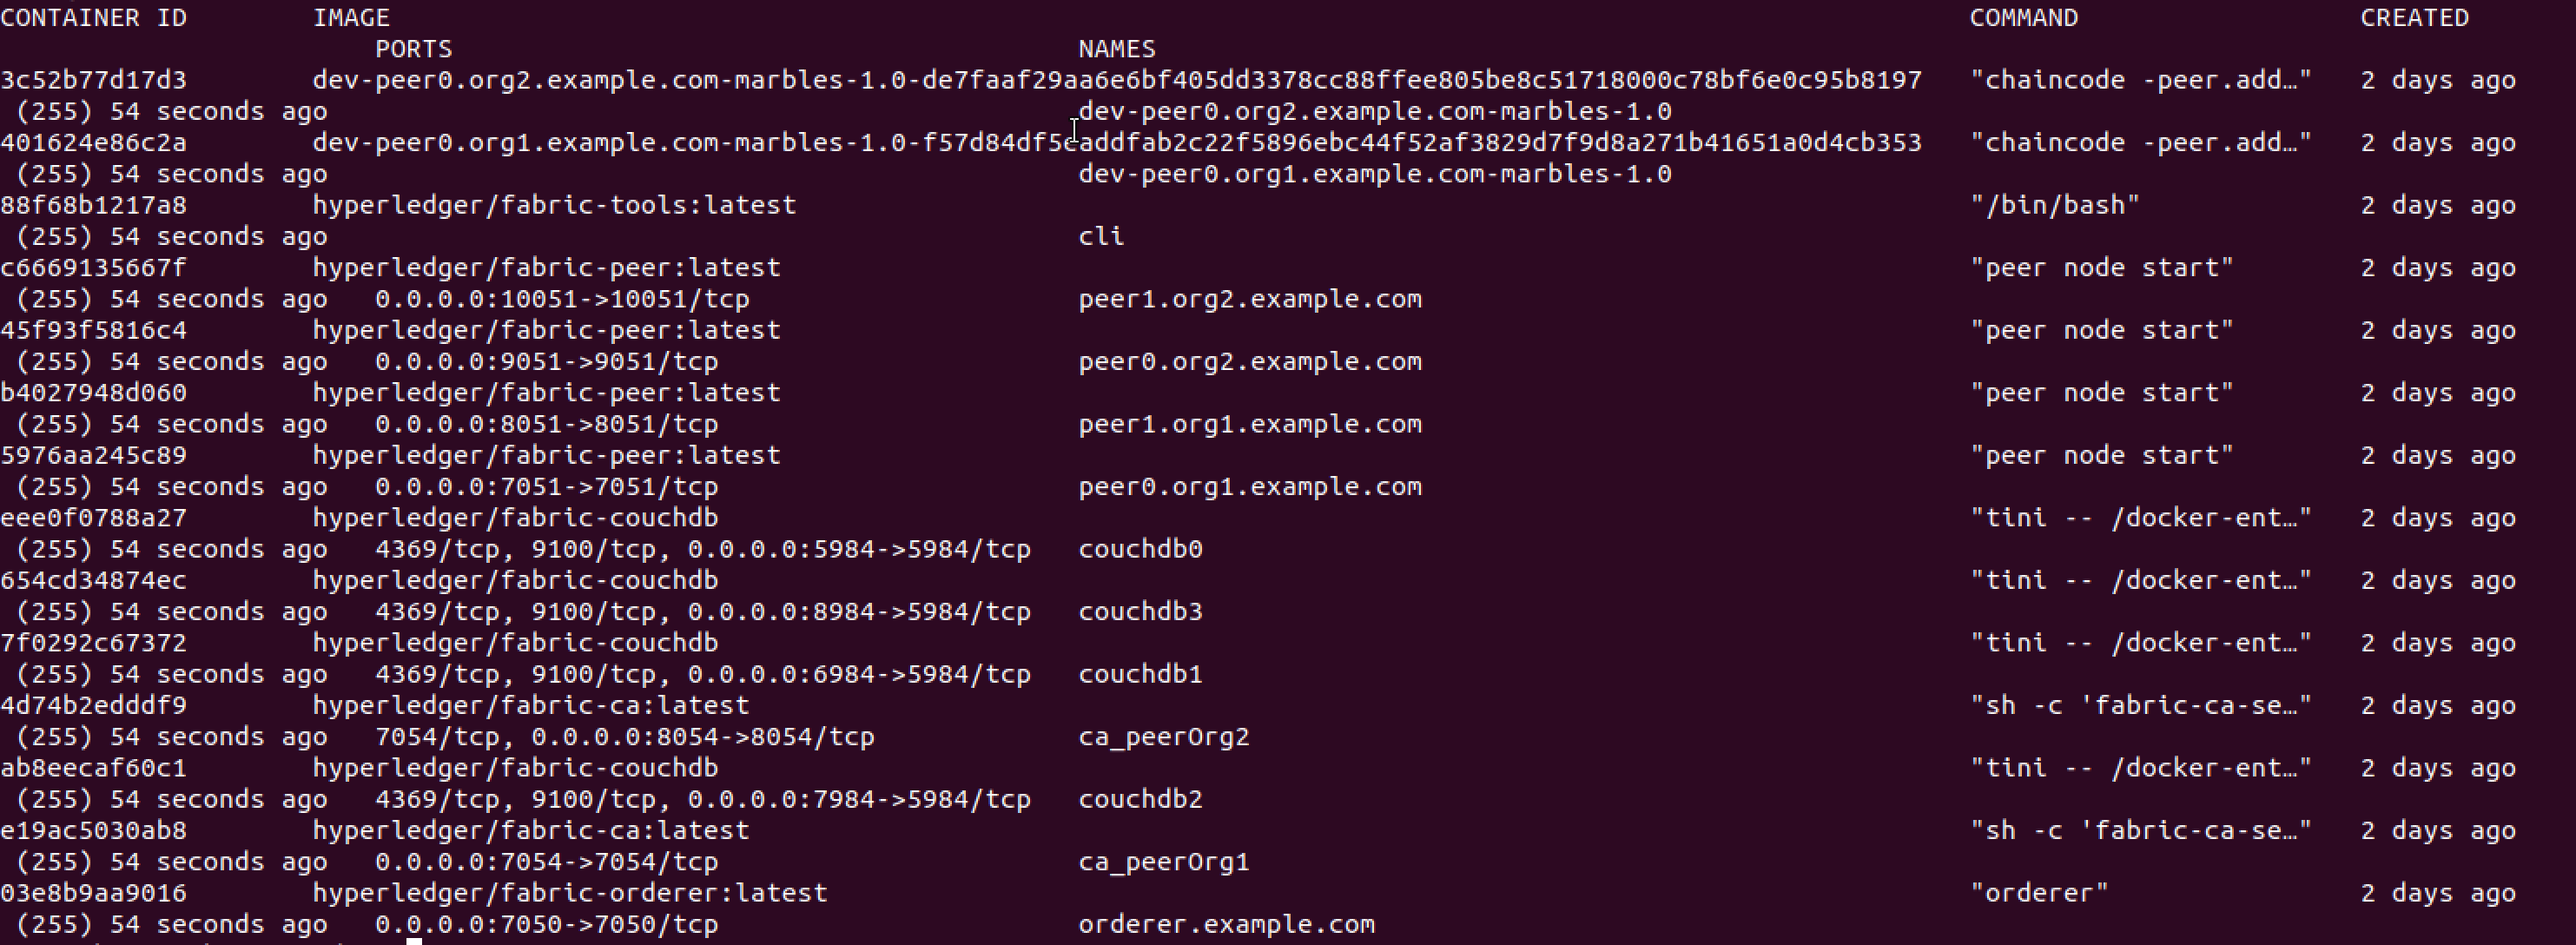
\includegraphics[width=1\textwidth]{img/docker-impl.png}
    \caption{Composizione dei container Docker per l'implementazione della rete blockchain}
    \label{fig:docker-impl}
\end{figure}
Gli script di inizializzazione lavorano in linguaggio shell, andando a definire una serie di comandi che inizializzano i container andando ad effettuare il caricamento delle applicazioni che montano le varie componenti sulla rete. 
Per entrambi i prototipi, la struttura di base è come quella appena descritta. Per eseguire l'inzi pt shell tramite un comando dal terminale Linux: 
\begin{verbatim}
    ./byfn.sh up -c mychannel -s couchdb
\end{verbatim}
L'esecuzione dello script di inizializzazione prende in input l'operazione da eseguire e due flag che definiscono il nome del canale da definire e la configurazione del tipo di database per mantenere le istanze dello stato globale del ledger sui vari peer di rete.
\subsection{File di configurazione}
Nello specifico, l'esecuzione consiste nel richiamare dei file di configurazioni in linguaggio YAML tramite il comando "docker-compose" in cui sono contenute le specifiche dei servizi da montare all'interno dei container. 
I tipi di file YAML implementati rappresentano delle policy strutturali che fanno riferimento ai seguenti concetti:
\begin{enumerate}
    \item Caratteristiche delle immagini delle componenti di base di un'organizzazione: MSP, Peer, autorità di certificazione, database di stato
    \item Configurazione della struttura del CA: Andando a definire le proprietà su cui si basano le autorità di certificazione
    \item Interfaccia a linea di comando: Definendo le proprietà dell'immagine dell'interfaccia a linea di comando da caricare. 
\end{enumerate}
Nei paragrafi successivi andremo ad analizzare ogni tipo di file YAML sotto un punto di vista implementativo. 
\subsubsection{File di configurazione delle immagini delle componenti di base}
\begin{figure}[h]
    \centering
    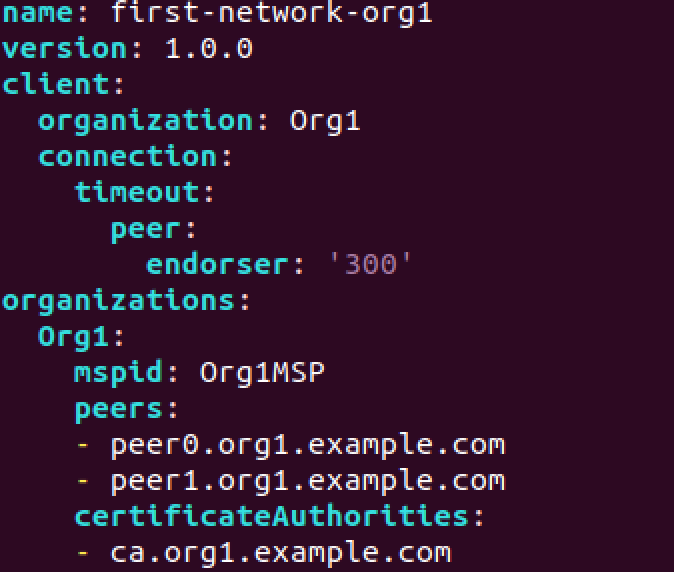
\includegraphics[width=0.5\textwidth]{img/connection-config-yaml.png}
    \caption{Snippet di codice YAML per la configurazione delle componenti di base di un'organizzazione mantenute nel file connection-org1.yaml}
    \label{fig:connection-config-yaml}
\end{figure}
Il file di configurazione delle immagini delle componenti di base di un'organizzazione è  definisce le proprietà per le seguenti entità di rete: 
\begin{itemize}
    \item Organizzazione: Consiste nelle specifiche dell'ID nominativo dell'entità, i riferimenti ai nomi dei peer, del CA e del MSP. 
    \item Peer: Consiste nelle specifiche dell'url, del nome logico, dei certificati di accesso e di opzioni del protocollo di comunicazione interno alla blockchain.
    \item CA: Consiste nelle specifiche dell'url, del nome di riferimento, del certificato di accesso e delle opzioni del protocollo di comunicazione con applicazioni esterne. 
\end{itemize}
All'interno dell'implementazione di entrambi i prototipi sviluppati, si è utilizzato il protocollo GRPC per la comunicazione interna e il protocollo HTTP per la comunicazione esterna che, nel nostro caso, fa riferimento ai server REST di interfacciamento alle funzioni delle istanze dei chaincode montate su ogni peer. 
\subsubsection{Configurazione della struttura del CA}
Il file YAML legato alla configurazione della struttura del CA definisce le proprietà dell'autorità di certificazione, le principali sono: 
\begin{itemize}
    \item Immagine su cui si basa ogni CA
    \item Variabili di Ambiente
    \item Porte di Comunicazione I/O
    \item Nome del Container
\end{itemize}
Mentre per la configurazione delle componenti di base si ha solamente la definizione delle componenti su cui agiscono i CA (certificati, host di accesso). All'interno della configurazione della loro struttura, si specificano tutte le proprietà logiche utilizzate per poter eseguire correttamente il meccanismo di autenticazione. Si è deciso di non distinguere il file di configurazione delle CA dandone solamente una definizione in modo che tutte le organizzazioni abbiano gli stessi meccanismi di accesso. 
\begin{figure}[h]
    \centering
    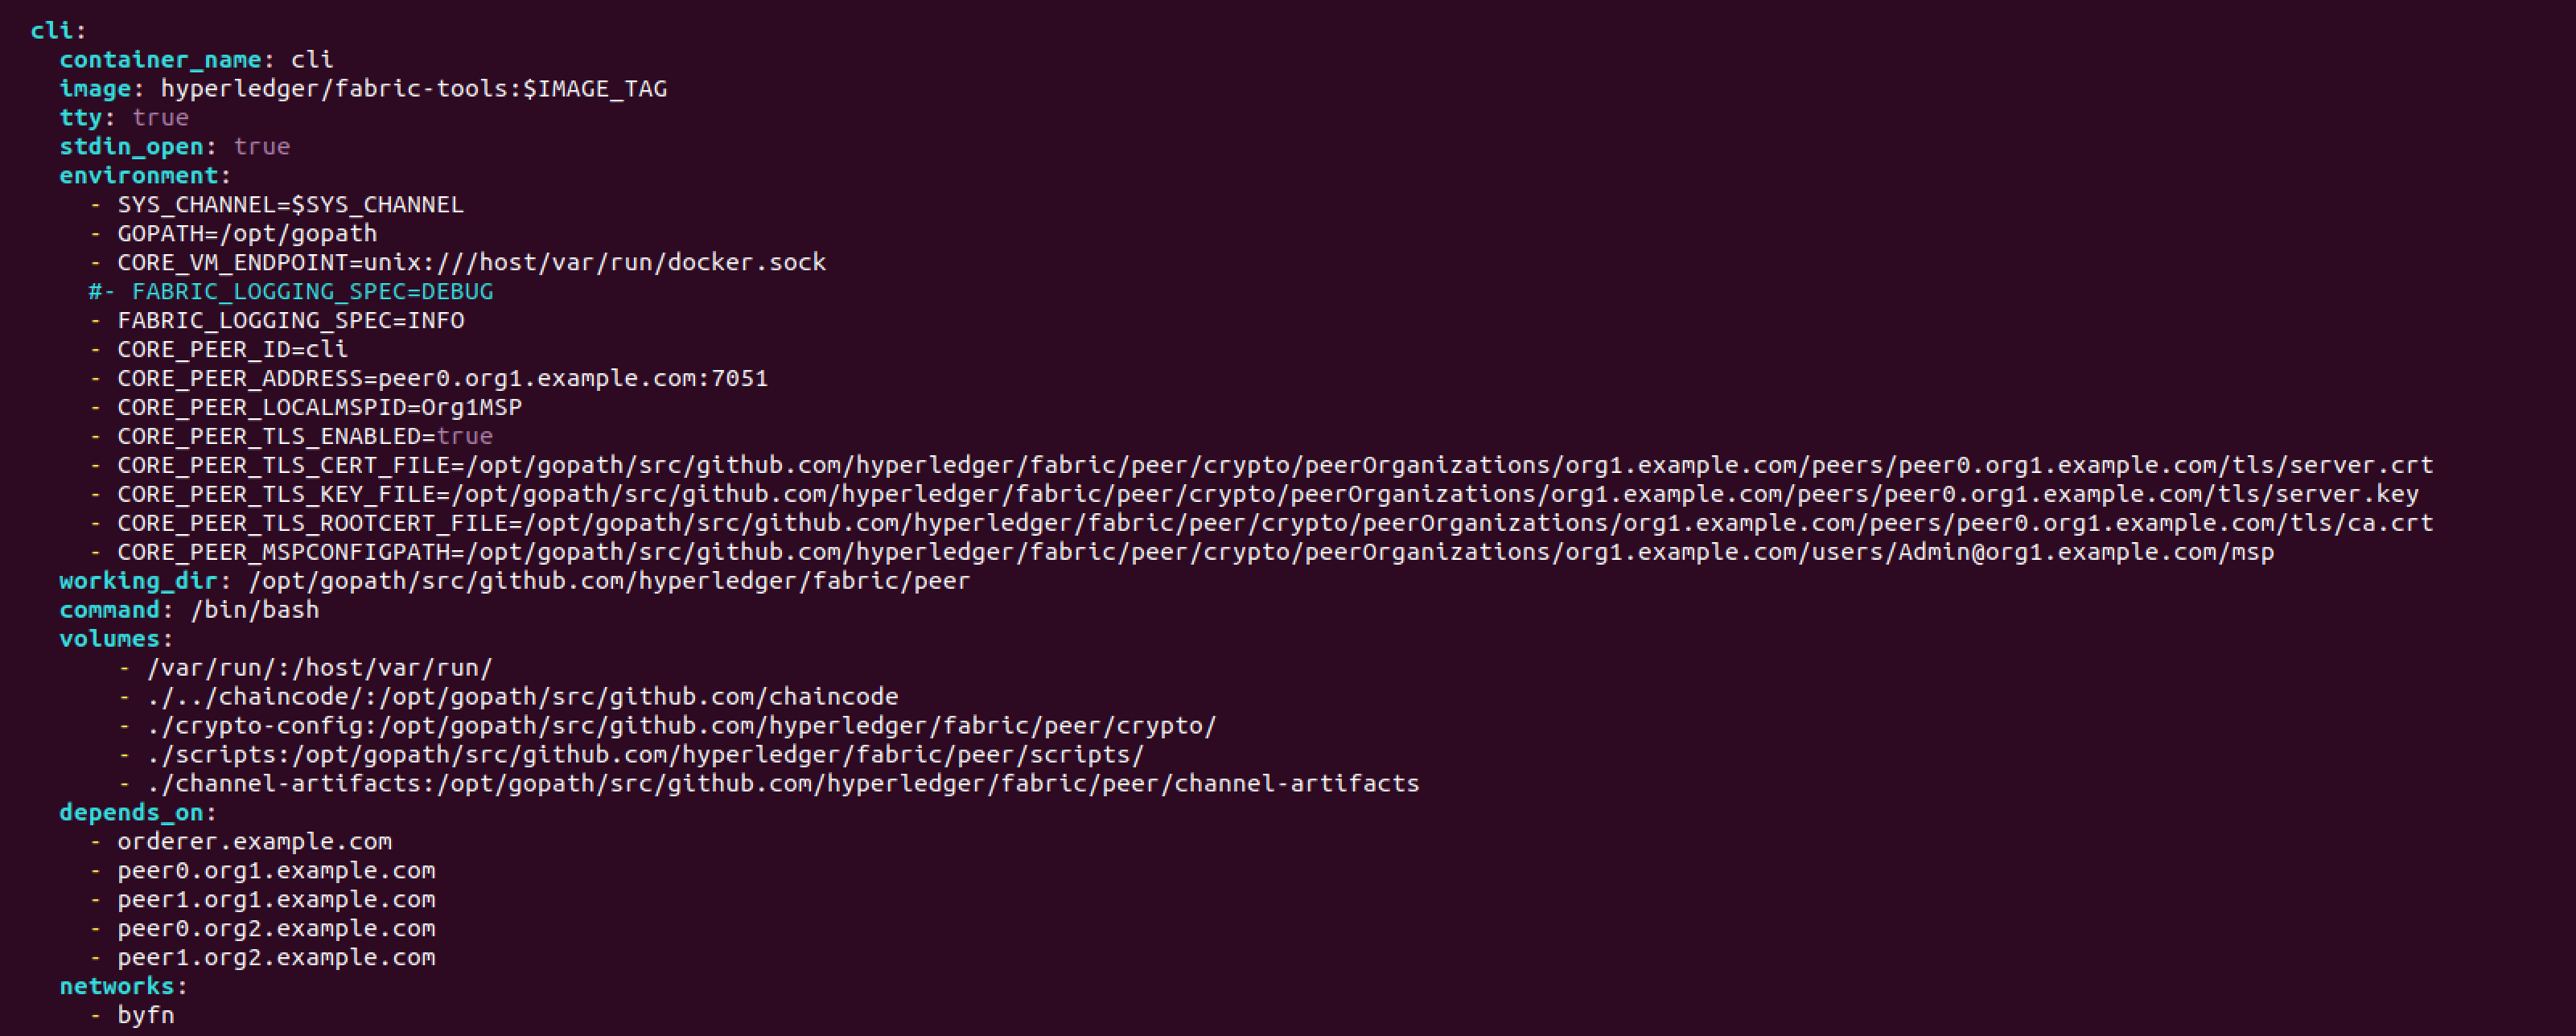
\includegraphics[width=1\textwidth]{img/docker-compose-cli-yaml.png}
    \caption{Snippet di codice YAML per la configurazione del CLI}
    \label{fig:connection-cli-yaml}
\end{figure}
\subsubsection{File di configurazione del CLI}
Il file YAML di configurazione del CLI della rete Fabric, denominato docker-compose-cli.yaml all'interno dei prototipi del progetto, è stato implementato  andando a specificare le seguenti proprietà: 
\begin{itemize}
    \item Nome del container
    \item Immagine del container
    \item Dipendenze
    \item Variabili di Ambiente
\end{itemize}
All'interno dei riferimenti ai volumi delle entità in cui può accedere il CLI, si ha che alcune proprietà  sono state isolate all'interno di un'ulteriore file di configurazione secondario chiamato "docker-compose-base.yaml" in cui poter trovare le caratteristiche di base dei servizi dipendenti come i peer di un'organizzazione o un'orderer.
\subsection{Gestione del chaincode}
Il chaincode viene definito tramite un file in linguaggio Golang istanziato in maniera distribuita sui vari peer delle organizzazioni partecipanti ad un canale sulla blockchain, la sua implementazione si concentra sulla definizione dei seguenti concetti: 
\begin{enumerate}
    \item Struttura delle collezioni di dati mantenute dentro lo stato globale del ledger
    \item Funzione di invocazione del chaincode
    \item Operazioni di business per la manipolazione dello stato globale
\end{enumerate}
\subsubsection{Struttura delle collezioni}
\begin{figure}[h]
    \centering
    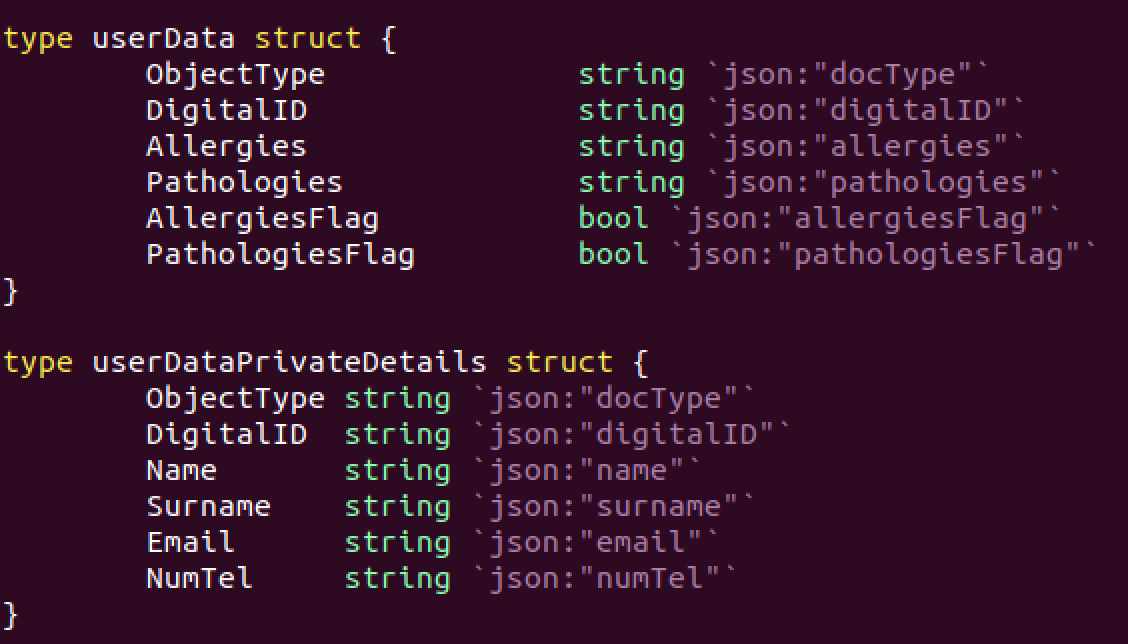
\includegraphics[width=0.8\textwidth]{img/collection-chaincode.png}
    \caption{Definizione della collezione all'interno del caso d'uso sanitario}
    \label{fig:collection-chaincode}
\end{figure}
\begin{figure}[h]
    \centering
    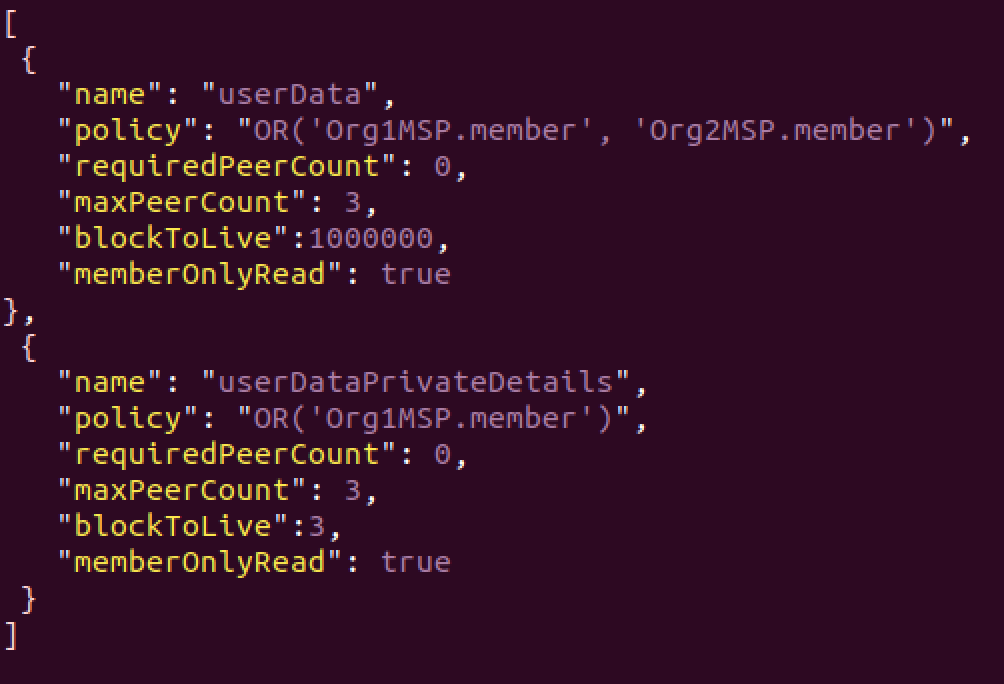
\includegraphics[width=0.8\textwidth]{img/policy-collection-json.png}
    \caption{Definizione delle policy di accesso per le collezioni del caso d'uso sanitario}
    \label{fig:policy-collection}
\end{figure}
In fase implementativa, le collezioni sono state definite come delle strutture dati globali.
Dentro il chaincode non vi è nessuna distinzione tra quali siano le collezioni private e quali pubbliche e nessun criterio di autorizzazione per verificare chi può o meno accedere, le politiche di gestione vengono specificate all'interno di un file di configurazione JSON esterno che definisce le policy di visibilità di una collezione. Tale file mantiene un array JSON in cui ogni elemento definisce i criteri di autenticazione specificati all'interno del paragrafo 3.5.2. Le collezioni private hanno un tempo di vita di blocco molto breve per evitare di andare a rendere reperibile i cambiamenti di stato tramite l'estrapolazione della storia della blockchain. Altre considerazioni implementative sono i riferimenti ai diritti di lettura in cui sono limitati solamente agli attori proprietari dei client d'interfacciamento, visibili dalla blockchain con il ruolo di membri semplici. Per la scrittura, invece, non vi sono limitazioni sui tipi di attori che possono effettuare tale operazione.

\newpage
\newpage
\subsubsection{Funzioni di invocazione}
\begin{figure}[h]
    \centering
    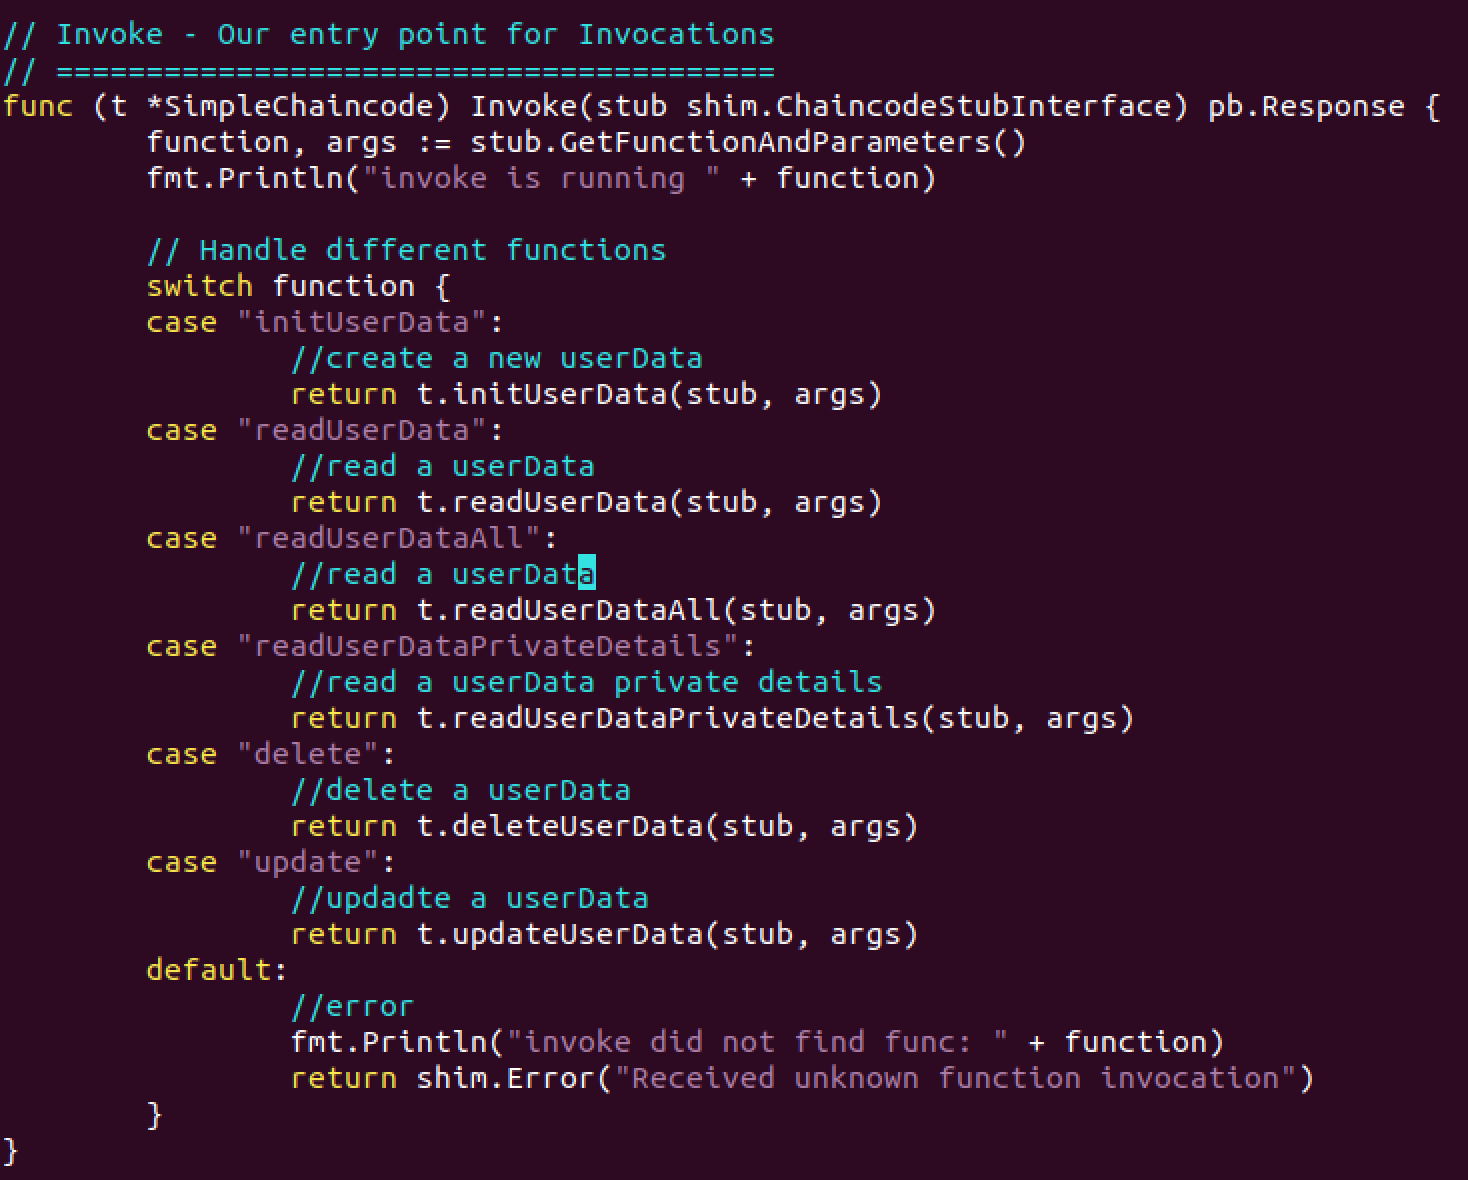
\includegraphics[width=0.8\textwidth]{img/invoke-chaincode.png}
    \caption{Funzione di invocazione nel chaincode della rete del prototipo sanitario}
    \label{fig:invoke-chaincode}
\end{figure}
La funzione d'invocazione nel chaincode viene richiamata ogni qualvolta si tende invocare un'operazione di business, l'implementazione di tale funzione prevede la gestione di inoltramento verso la chiamata della funzione del chaincode corrispondente andando a inoltrare l'interfaccia stub del chaincode e i parametri di input. La funzione GetFunctionAndParameters viene utilizzata per prendere i campi corrispondenti all'interno della struttura della request della REST API attraverso lo stub del chaincode. La libreria shim ha anche delle funzioni di controllo sulla richiesta che possono definire l'identità del chiamante e andare ad analizzare il suo ID per poter decidere già all'interno di tale funzione se un client sia autorizzato o meno. Nel caso dei prototipi, invece, si accede alla funzione e si controlla l'autorizzazione solamente quando si invocano le funzioni di alterazione o di accesso dello stato globale del ledger, ossia quando si accede alla copia del couchdb del peer richiamato.
\newpage
\subsubsection{Operazioni di business}
Le operazioni di business sono state implementate tramite varie funzioni che possono essere categorizzate in due grandi tipi: lettura e scrittura. Se l'operazione è di lettura, si riceve in input l'ID corrispondenti ad un oggetto JSON salvato all'interno del couchdb rappresentante lo stato globale del ledger. Se l'operazione è di scrittura, si riceve in input una struttura dati corrispondente ai dati delle collezione da sovrascrivere. L'operazione di modifica si identifica come un'operazione di scrittura in cui si ha la sovrascrizione dei dati di un particolare oggetto JSON salvato all'interno dello stato globale. Questa peculiarità ha come risultato quello di poter visualizzare, all'interno della storia del ledger, tutte le sovrascrizioni effettuate su un particolare oggetto a secondo del tempo di vita del blocco specificato dentro il file di configurazione della collezione di cui fa parte. Per quanto riguarda gli output delle funzioni, se l'operazione è di lettura si ritornano i dati letti dal ledger altrimenti, nel caso di un'operazione di scrittura, si darà in output un valore di stato che differisce a secondo se la procedura è andata a buon fine o meno.
\begin{figure}[h]
    \centering
    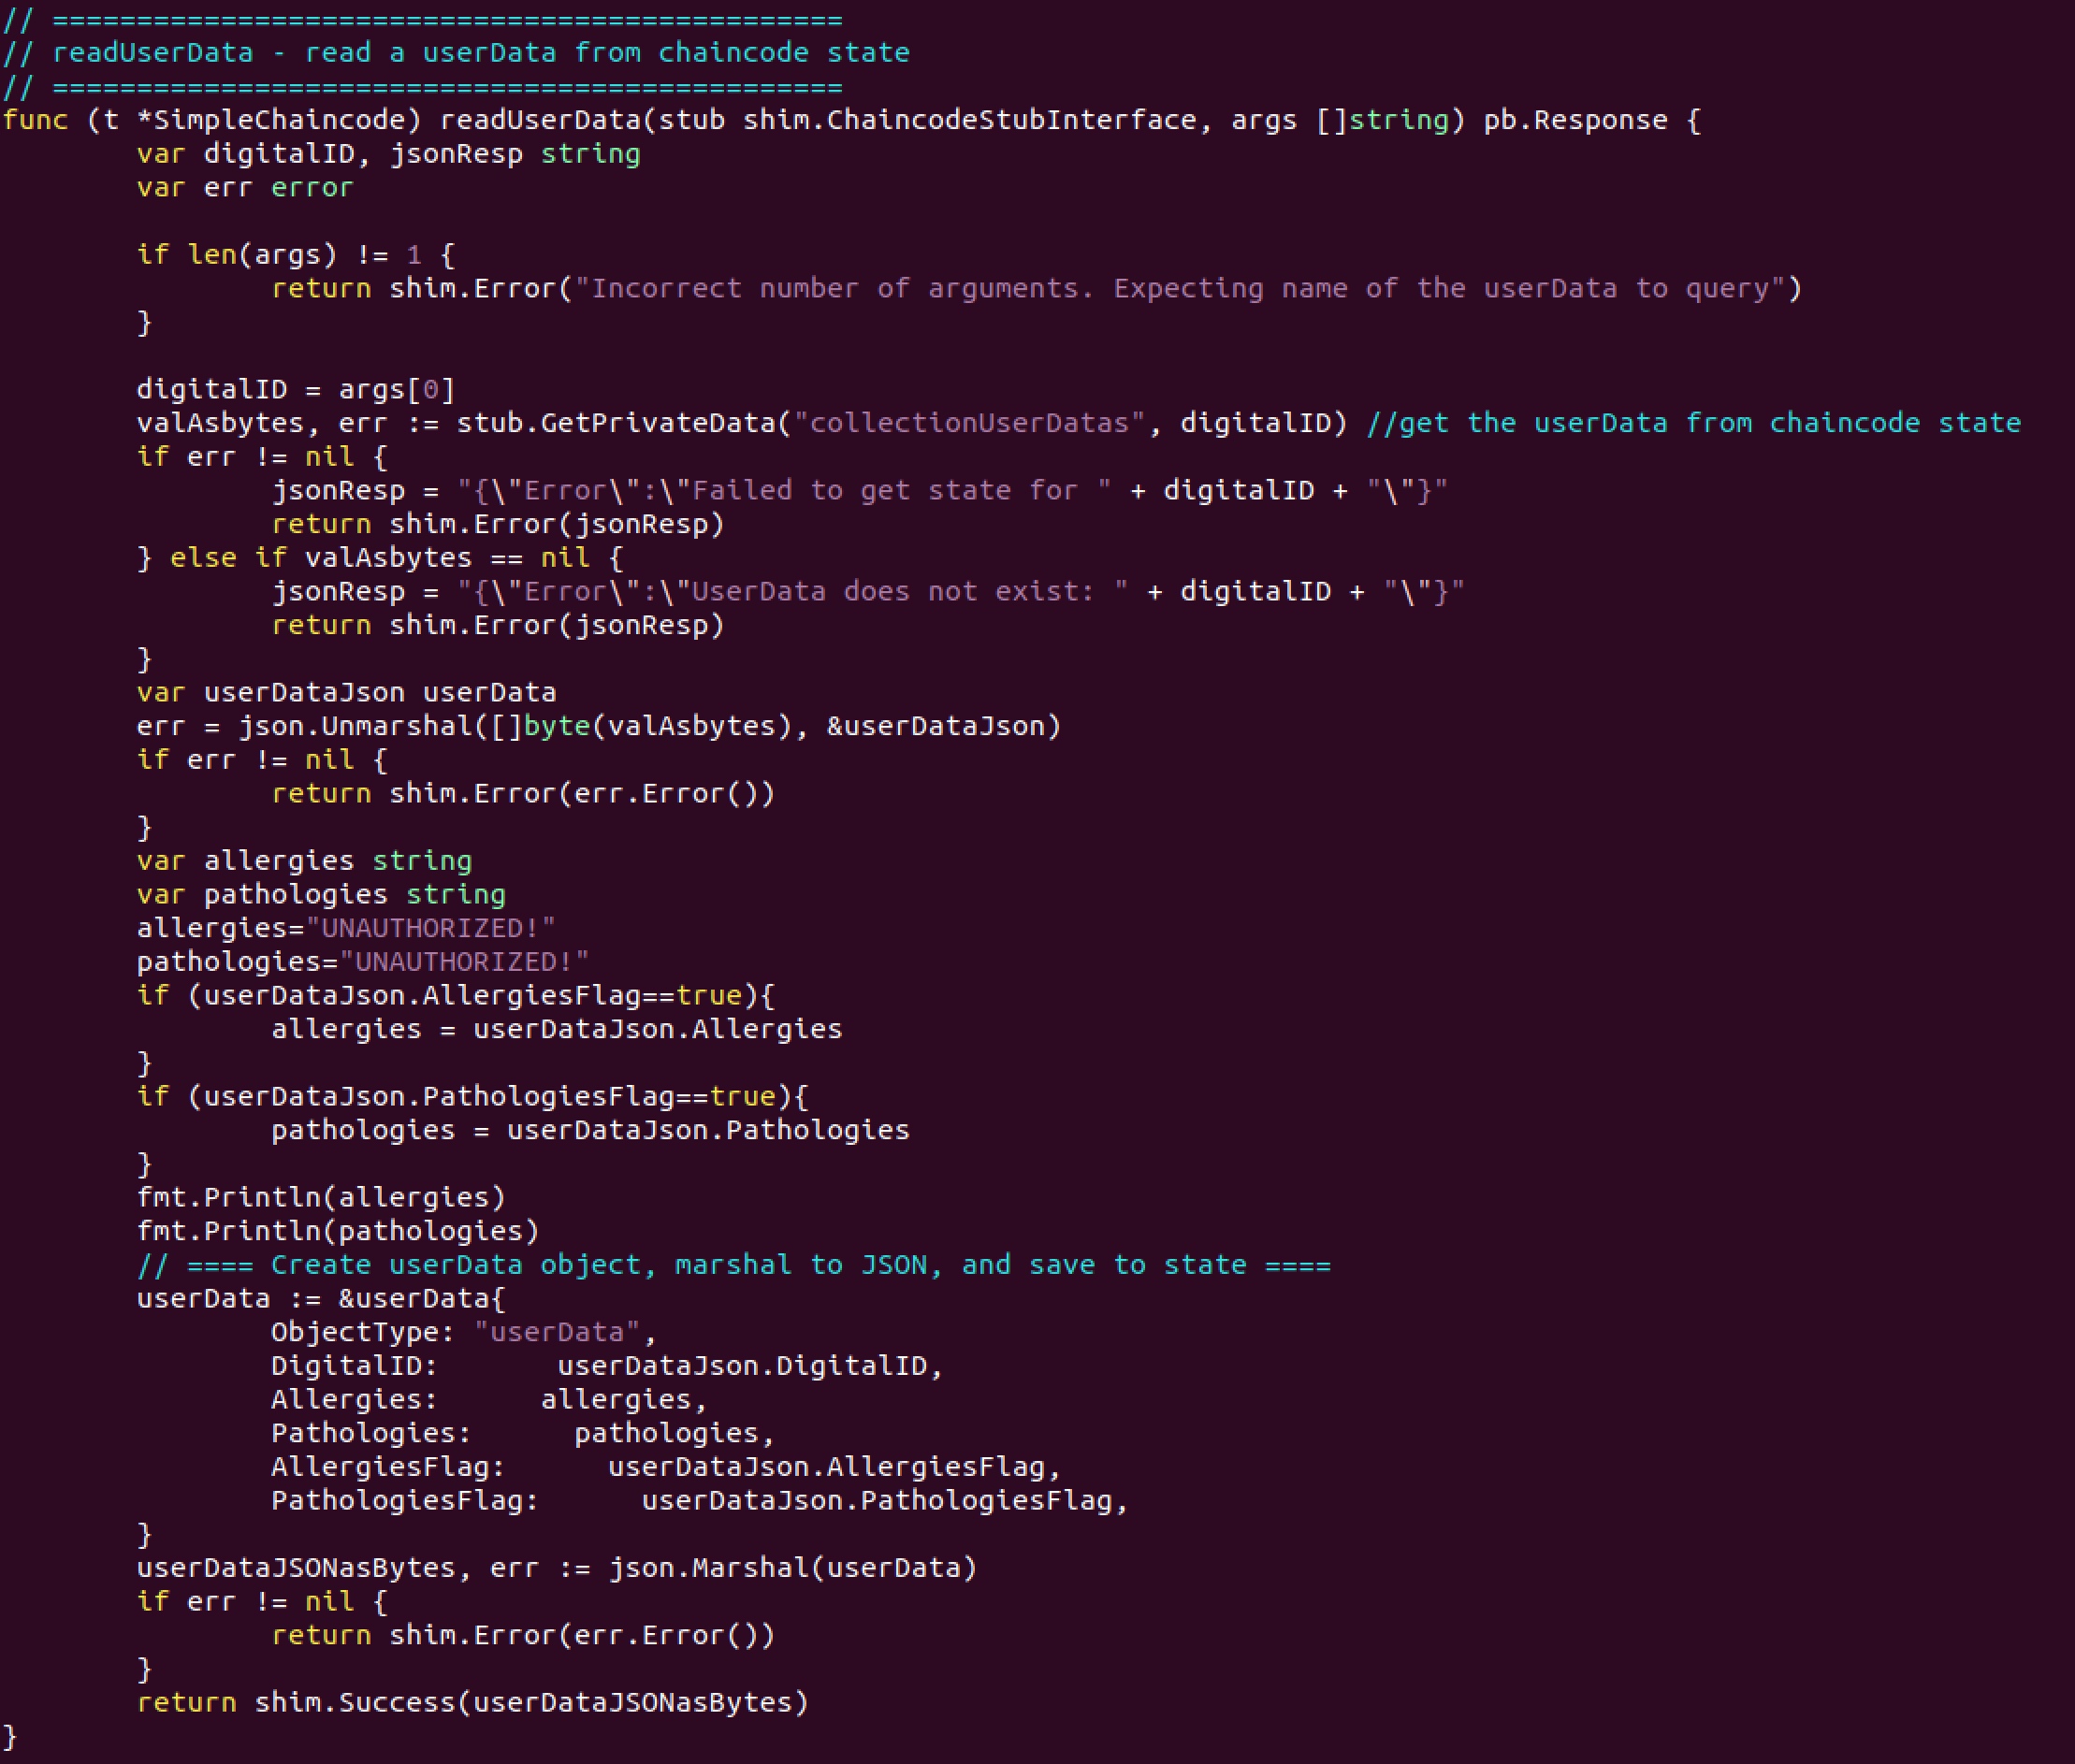
\includegraphics[width=1\textwidth]{img/function-chaincode.png}
    \caption{Funzione di lettura dei dati pubblici nel chaincode del caso sanitario}
    \label{fig:function-chaincode}
\end{figure}
\newpage
\section{Evoluzione del progetto}
Partendo dai prototipi sviluppati, possiamo ipotizzare che il prossimo step implementativo sia quello di adattare l'architettura formata da due organizzazioni a una più affine alla gestione logica degli attori dei due casi d'uso, andando a specificare un'organizzazione per ogni tipo di attore. Altre caratteristiche da poter migliorare sono quelle legate al sistema d'identificazione e di autenticazione andando a sostituire gli UUID autogenerati del prototipo con ID generati da un servizio di riconoscimento facciale.
\newpage